\begin{figure}[tbp]
\centering
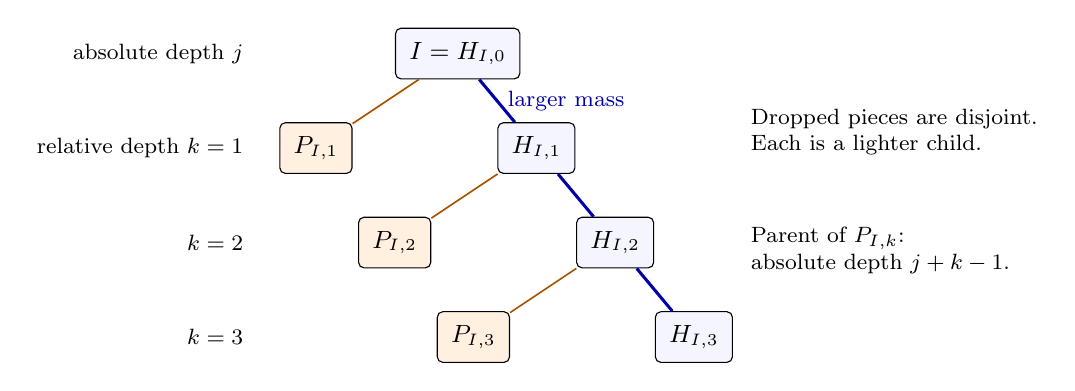
\begin{tikzpicture}[
  interval/.style={draw,rounded corners=2pt,inner sep=5pt,
                   fill=blue!4,font=\small},
  lighter/.style={draw,rounded corners=2pt,inner sep=5pt,
                  fill=orange!12,font=\small},
  heavyedge/.style={line width=1.1pt,blue!65!black},
  lightedge/.style={line width=.6pt,orange!65!black},
  note/.style={font=\footnotesize,align=left}
]
\node[interval] (root) at (0,0) {$I=H_{I,0}$};
\node[lighter] (p1) at (-1.8,-1.2) {$P_{I,1}$};
\node[interval] (h1) at (1.0,-1.2) {$H_{I,1}$};
\node[lighter] (p2) at (-.8,-2.4) {$P_{I,2}$};
\node[interval] (h2) at (2.0,-2.4) {$H_{I,2}$};
\node[lighter] (p3) at (.2,-3.6) {$P_{I,3}$};
\node[interval] (h3) at (3.0,-3.6) {$H_{I,3}$};
\draw[lightedge] (root)--(p1);
\draw[heavyedge] (root)--node[right,note] {larger mass}(h1);
\draw[lightedge] (h1)--(p2);
\draw[heavyedge] (h1)--(h2);
\draw[lightedge] (h2)--(p3);
\draw[heavyedge] (h2)--(h3);
\node[note,anchor=east] at (-2.6,0) {absolute depth $j$};
\node[note,anchor=east] at (-2.6,-1.2) {relative depth $k=1$};
\node[note,anchor=east] at (-2.6,-2.4) {$k=2$};
\node[note,anchor=east] at (-2.6,-3.6) {$k=3$};
\node[note,anchor=west] at (3.6,-1.0)
  {Dropped pieces are disjoint.\\
   Each is a lighter child.};
\node[note,anchor=west] at (3.6,-2.5)
  {Parent of $P_{I,k}$:\\
   absolute depth $j+k-1$.};
\end{tikzpicture}
\caption{Three steps of the heavier-child path.  At each step the
 lighter sibling is set aside; the chosen child is split again.  The
 dropped siblings together with the terminal child partition $I$.
 For fixed relative depth $k$, changing the frequency index $j$ changes
 the absolute depth of the parent.  This makes the parents distinct in
 the sum controlled by the convexity deficit.}
\label{fig:endpoint-tree}
\end{figure}
